There are two reactor models created - Sangamon200, a 200MWth design inspired by the PBMR and Xe-100.  Using data from the Sangamon200 model, a scaled down reactor called the Sangamon20 was created.  Both are UCO-pebble fueled, helium cooled microreactors.

\begin{table}[h!]
\centering
\caption{Geometric and Internal Core Parameters in the Sangamon Reactors}
\begin{tabular}{ c  c  c }
\hline
Parameter & Sangamon200 \cite{harlan_x-energy_2018}, \cite{harlan_ans_2017} & Sangamon20 \\
\hline
Thermal Power [MW] & 200 & 20 \\
Average Core Temperature [K] & 800 & 800 \\
Enrichment [wt\%] & 15.5\% & 19.75\% \\
Average Core Pressure [MPa] & 5.9 & 5.9 \\
Outer Core Radius [cm] & 216 & 165 \\
Outer Core Height [cm] & 1150 & 330 \\
Reflector Thickness [cm] & 92 & 75 \\
Number of Pebbles & 220,000 & 22,680 \\
Packing Fraction [\%] & 53.0 & 56.0 \\
\hline
\end{tabular}

\label{table:params1}
\end{table}

All simulations were performed using Serpent 2.0 \cite{leppanenjaakko_serpent_2015}.  Pebble and TRISO particle locations are both determined using the Serpent 2.0 particle dispersal routine.  In Serpent 2.0, the particle dispersal algorithm first takes the number of particles, defined by the user directly, or indirectly using $\eta_{pf}$, the packing fraction, which is simply the total volume of particles in a space divided by the volume of that space.  The dispersal routine also has the user define the particle radius, and the size and shape of the volume the particles are housed in.  The routine first randomly determines a single point for each particle that is contained in the volume.  Then, the routine uses the 'growth factor' and 'shake factor' - both described as fractions of the particle radius, and iterates.  Each iteration, the size of the point's radius increases by the growth factor.  Additionally, the center will move in a random direction a distance equal to the shake factor.  If the particle growth would cause the particle to overlap with another particle or leave the volume, it doesn't get larger that cycle.  Similarly, if the center's movement would cause overlap or leaving the containing volume, it doesn't move.  The dispersal routine iterates until all particles are to their full size, contained in the volume, and do not overlap with any other particles.  The routine generates an output file, where each line gives the coordinates of the particle center in x,y,z coordinates, the particle radius, and the name of the particle type, to associate it with the pbed card later.
\\ \\

In order to determine isotopic compositions in the pebbles, a Serpent burnup simulation of a single pebble is run in burnup steps of 180, 360, 540, 720, 900, and 1080 days - to represent 6, 6-month passes.  A seventh composition is for a fresh pebble's composition.  The single pebbles are the only models that utilize individually modeled TRISO particles.  For the full-core models, each pebble is  homogenized.  Each pebble has two regions, an inner region that contains the TRISO particles embedded in graphite, and an outer region consisting only of graphite, see \ref{fig:pebb-zone1}.  Each region is homogenized by volume fraction using the mix card in Serpent.

\begin{figure}[H]
\centering


\includegraphics[width=0.5\linewidth]{figures/pebble-zones.png}
\caption{Pebble Zones}
\label{fig:pebb-zone1}
\end{figure}


\begin{table}[h!]
\centering

\caption{Pebble Parameters}
\begin{tabular}{ c  c }
\hline
Parameter & Value \\
\hline
Fueled-Center Radius [cm] & 2.5 \\
Graphite Outer Shell Thickness [cm] & 0.5 \\
Total Radius [cm] & 3.0 \\
TRISO Particles per Pebble & 18,000 \\
\hline
\end{tabular}
\label{table:peb-params}
\end{table}


\begin{figure}[H]
\centering

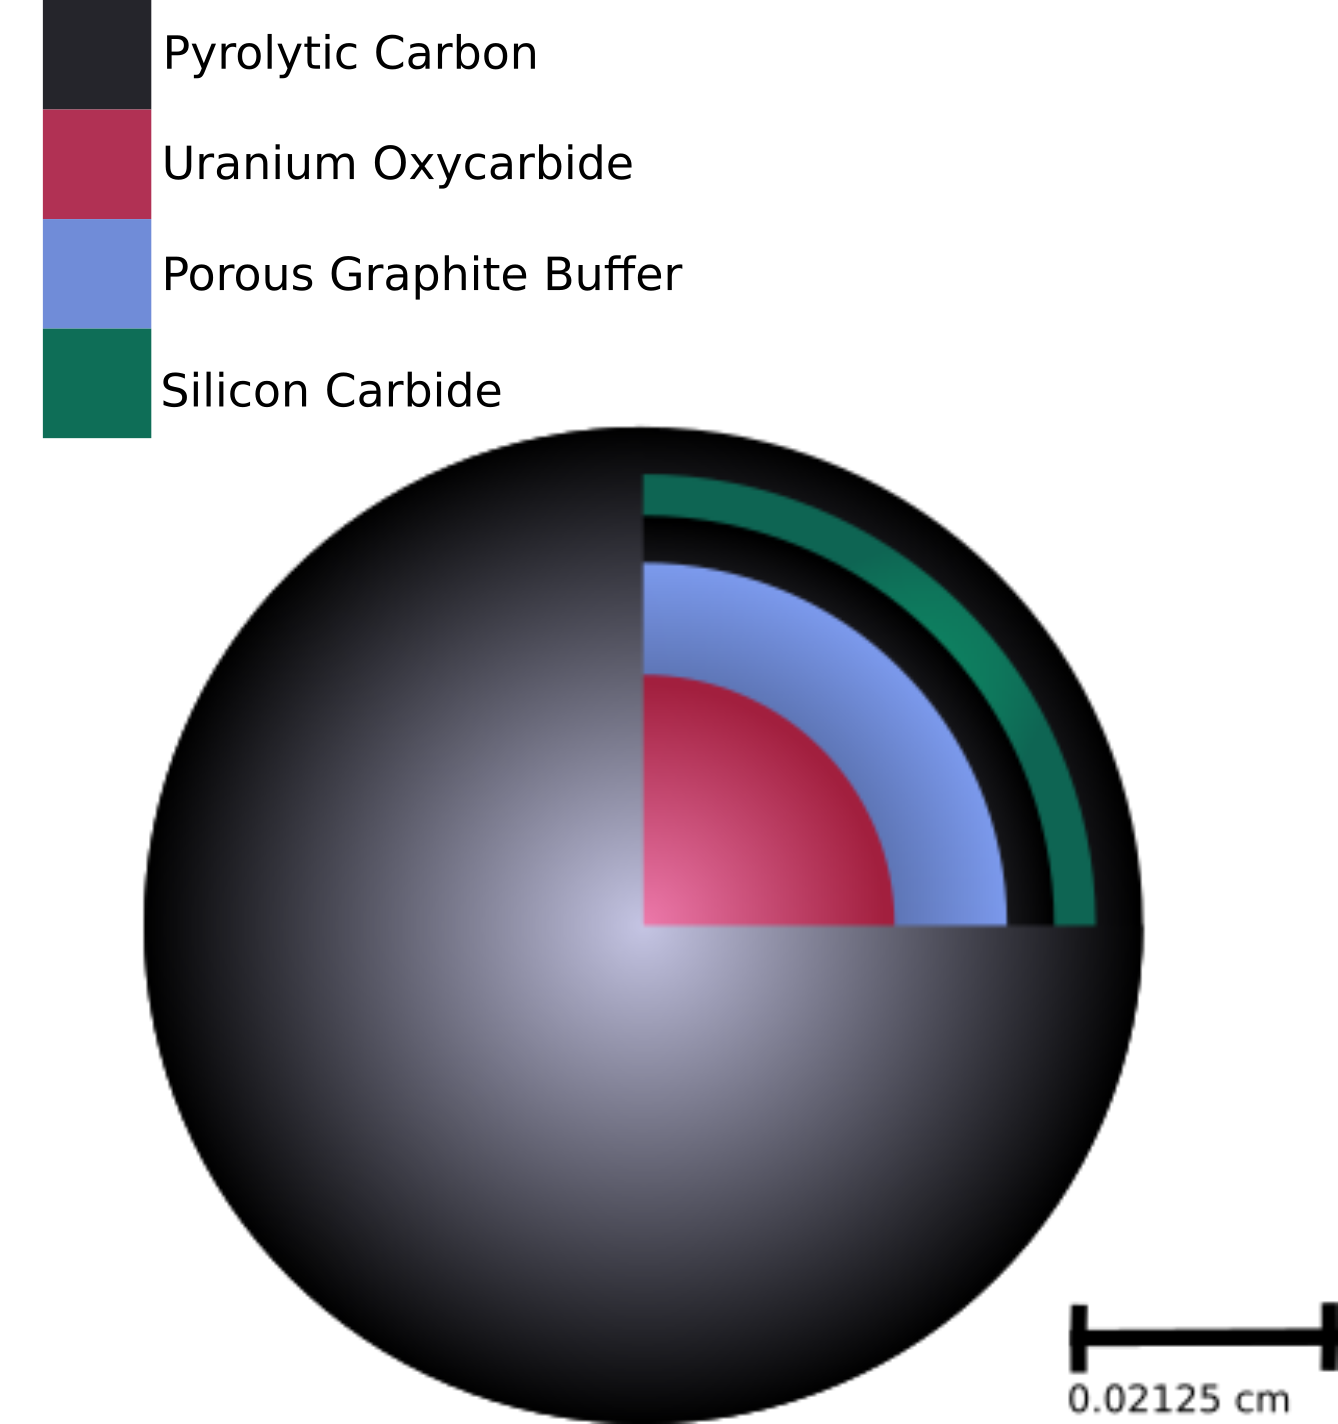
\includegraphics[width=0.5\linewidth]{figures/trisos-r-like-onions.png}
\caption{TRISO Particle Layers}
\label{fig:particle-layer}
\end{figure}

\begin{table}[h!]
\centering

\caption{Particle Parameters Used in Monte Carlo Simulations}
\begin{tabular}{ c  c }
\hline
Parameter & Value [cm] \\
\hline 
Uranium Oxycarbide Kernel Radius & 0.02125 \\
Graphite Layer Thickness & 0.03075 \\
Inner Pyrolytic Carbon Layer Thickness & 0.03475 \\
Silicon Carbide Layer Thickness & 0.03825 \\
Outer Pyrolytic Carbon Layer Thickness & 0.04225 \\
\hline
\end{tabular}
\label{table:particle-params}

\end{table}

\begin{table}[h!]
\centering
\begin{tabular}{ c  c }
\hline
Parameter & Value \\
\hline
Fueled-Center Radius [cm] & 2.5 \\
Graphite Outer Shell Thickness [cm] & 0.5cm \\
Total Radius [cm] & 3.0 \\
TRISO Particles per Pebble & 18,000 \\
\hline
\end{tabular}
\caption{Pebble Parameters}
\label{table:params2}
\end{table}
\begin{table}[h!]
\centering
\begin{tabular}{|| c || c |}
\hline
Parameter & Value \\
\hline \hline
Uranium Oxycarbide Kernel Radius [cm] & 0.02125 \\
Graphite Layer Thickness [cm] & 0.03075 \\
Inner Pyrolytic Carbon Layer Thickness [cm] & 0.03475 \\
Silicon Carbide Layer Thickness [cm] & 0.03825 \\
Outer Pyrolytic Carbon Layer Thickness [cm] & 0.04225 \\
\hline
\end{tabular}
\caption{Particle Parameters}
\label{table:params3}
\end{table}


\section{Sangamon200}
Sangamon200 is a 200 MWth helium cooled reactor, with parameters as defined in \ref{table:params1}.  Though the model does use some parameters from pre-established designs, it is still, a simplification.  The "cone" formed at the top and bottom of the reactor core by the pebbles  is averaged to a flat surface, to create a cylindrical core shape.  The graphite reflector surrounds it, with no barriers between the reflector and helium/pebble-filled active core region.  In effect, the reflector is the container for the pebbles.  These are the only simulated parts of the reactor.  It is assumed no control rods are being used.  In addition, the graphite reflector is defined as a solid cylindrical shell.

While Sangamon200 is not the focus of this assessment, some neutronics features were determined to aid in Sangamon20's design.  A surface current detector was placed in the reflector, just inside the outer bound of the reflector, as shown in \ref{fig:det-place}.

\begin{figure}[H]
\centering
\resizebox{0.5\textwidth}{!}{%
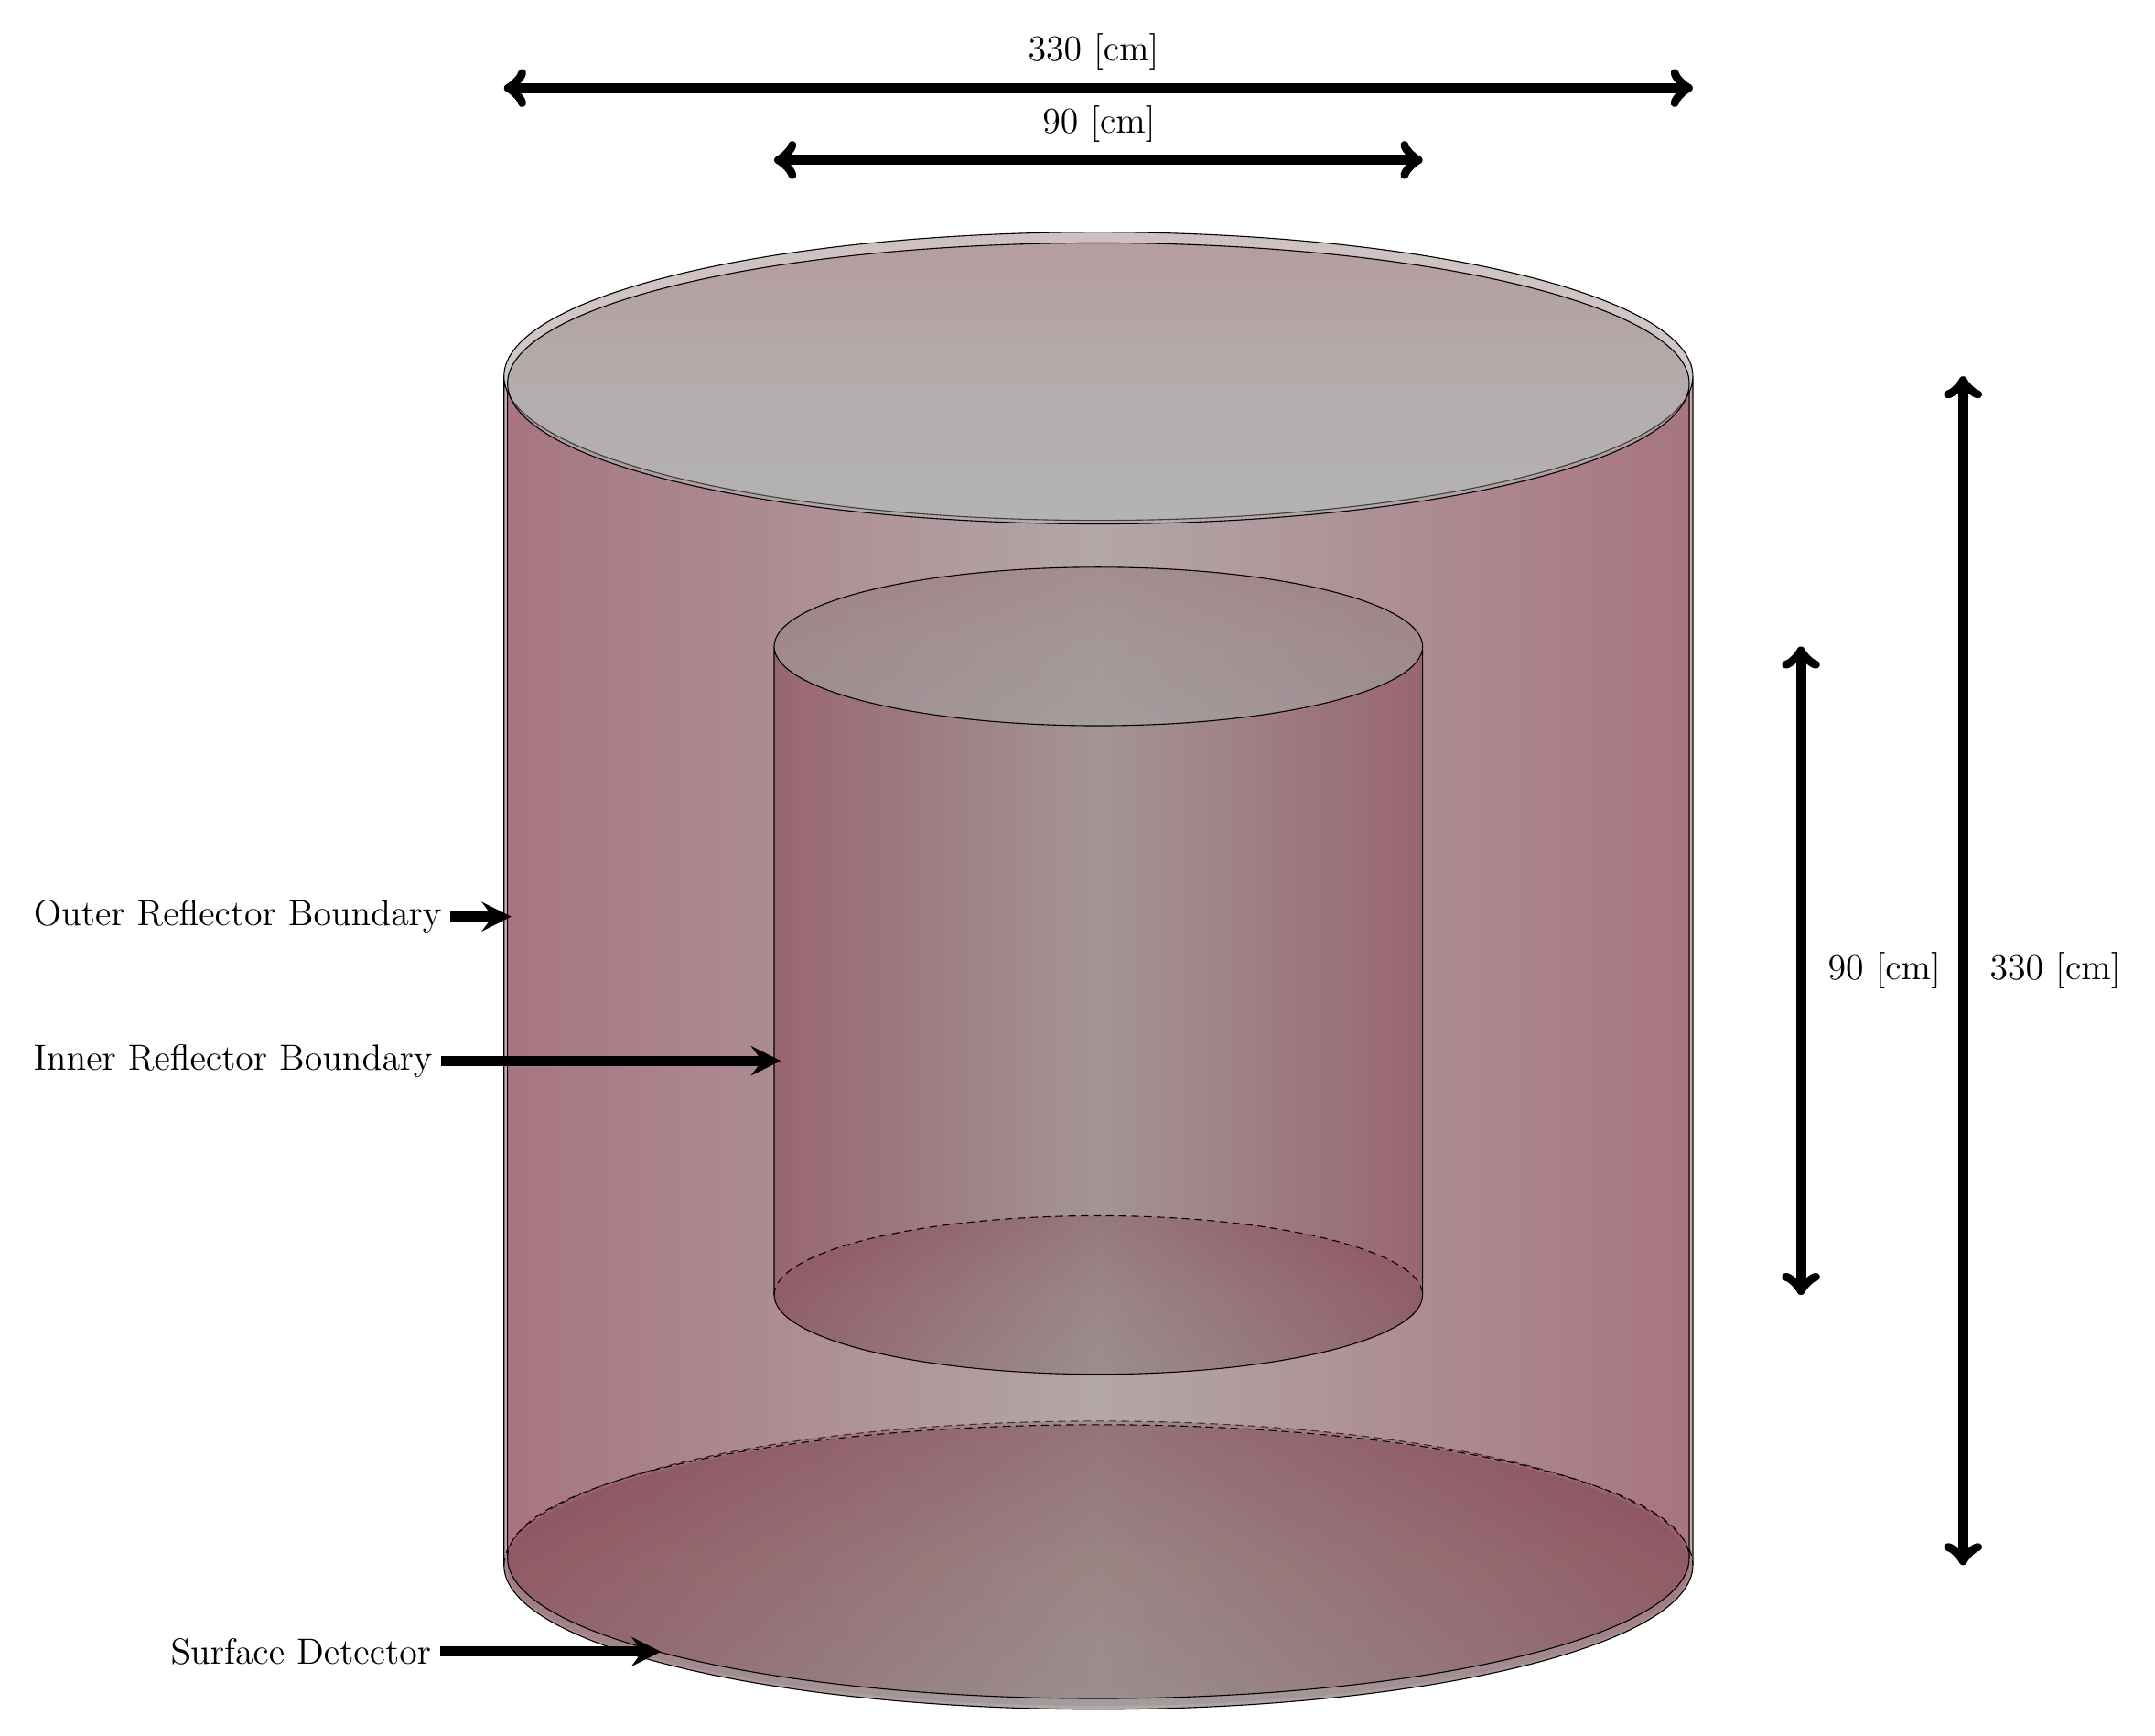
\begin{tikzpicture}
\fill[top color=pink!50!purple,bottom color=pink!10,middle color=pink,shading=axis,opacity=0.25] (0,0) circle (8.25cm and 2.0cm);
\fill[left color=pink!50!purple,right color=pink!50!purple,middle color=pink!50,shading=axis,opacity=0.25] (8.25,0) -- (8.25,16.5) arc (360:180:8.25cm and 2.0cm) -- (-8.25,0) arc (180:360:8.25cm and 2.0cm);
\fill[top color=pink!90!,bottom color=pink!2,middle color=pink!30,shading=axis,opacity=0.25] (0,16.5) circle (8.25cm and 2.0cm);
\draw (-8.25,16.5) -- (-8.25,0) arc (180:360:8.25cm and 2.0cm) -- (8.25,16.5) ++ (-8.25,0) circle (8.25cm and 2.0cm);
\draw[densely dashed] (-8.25,0) arc (180:0:8.25cm and 2.0cm);

\fill[top color=pink!50!purple,bottom color=pink!10,middle color=pink,shading=axis,opacity=0.25] (0,0.0) circle (8.2cm and 1.95cm);
\fill[left color=pink!50!purple,right color=pink!50!purple,middle color=pink!50,shading=axis,opacity=0.25] (8.2,0.1) -- (8.2,16.4) arc (360:180:8.2cm and 1.95cm) -- (-8.2,0.1) arc (180:360:8.2cm and 1.95cm);
\fill[top color=pink!90!,bottom color=pink!2,middle color=pink!30,shading=axis,opacity=0.25] (0,16.4) circle (8.2cm and 1.95cm);
\draw (-8.2,16.3) -- (-8.2,0.1) arc (180:360:8.2cm and 1.95cm) -- (8.2,16.3) ++ (-8.2,0.1) circle (8.2cm and 1.95cm);
\draw[densely dashed] (-8.2,0.1) arc (180:0:8.2cm and 1.85cm);

\fill[top color=pink!50!purple,bottom color=pink!10,middle color=pink,shading=axis,opacity=0.25] (0,3.75) circle (4.5cm and 1.1cm);
\fill[left color=pink!50!purple,right color=pink!50!purple,middle color=pink!50,shading=axis,opacity=0.25] (4.5,3.75) -- (4.5,12.75) arc (360:180:4.5cm and 1.1cm) -- (-4.5,3.75) arc (180:360:4.5cm and 1.1cm);
\fill[top color=pink!90!,bottom color=pink!2,middle color=pink!30,shading=axis,opacity=0.25] (0,12.75) circle (4.5cm and 1.1cm);
\draw (-4.5,12.75) -- (-4.5,3.75) arc (180:360:4.5cm and 1.1cm) -- (4.5,12.75) ++ (-4.5,3.75) (0,12.75) circle (4.5cm and 1.1cm);
\draw[densely dashed] (-4.5,3.75) arc (180:0:4.5cm and 1.1cm);

\node [anchor=west] (out-ref) at (-14.9, 9) {\Large Outer Reflector Boundary};
\node [anchor=west] (in-ref) at (-14.9, 7) {\Large Inner Reflector Boundary};
\node [anchor=west] (det) at (-13, -1.2) {\Large Surface Detector};

\draw [-stealth, line width=4pt, black] (out-ref) -- ++(3.8,0);
\draw [-stealth, line width=4pt, black] (in-ref) -- ++(7.6,0);
\draw [-stealth, line width=4pt, black] (det) -- ++(5.0,0);

\draw [-stealth, <->, line width=4pt, black] ++(-8.25,20.5) -- ++(16.5,0);
\draw [-stealth, <->, line width=4pt, black] ++(12,0) -- ++(0,16.5);

\node [anchor=west] (out-h) at (12.25, 8.25) {\Large 330 [cm]};
\node [anchor=west] (out-d) at (-1.1, 21.0) {\Large 330 [cm]};

\draw [-stealth, <->, line width=4pt, black] ++(-4.5,19.5) -- ++(9,0);
\draw [-stealth, <->, line width=4pt, black] ++(9.75,3.75) -- ++(0,9.0);

\node [anchor=west] (in-h) at (10.0, 8.25) {\Large 90 [cm]};
\node [anchor=west] (in-d) at (-0.9, 20.0) {\Large 90 [cm]};

\end{tikzpicture}
 }%
\caption{Detector Placement Inside Reflector in Sangamon200 and Sangamon20}
\label{fig:det-place}

\end{figure}


This detector measures the outward neutron current (*** serpent outputs units of [number/s], is current still the best word? ***) in $[\frac{\#}{s}]$.  To arrive at the unit of $[\frac{\#}{cm^2s}]$ most are familiar with, the reported outward current is divided by the detector's surface area thus:
\begin{equation}
J^+ [\frac{\#}{cm^2s}] = \frac{J^+ [\frac{\#}{s}]}{S_{det}[cm^2]}
\end{equation}

After accounting for the surface area, the outward current at the detector is $7.351x10^{11}$.

\section{Sangamon20}

Sangamon20 is a 20 MWth helium-cooled pebble bed reactor, fueled with 19.75\% enriched uranium oxycarbide.  While the capacity of Sangamon20 is 10\% that of Sangamon200, it isn't sufficient to simply scale Sangamon200's dimensions down to 10\% of their original values, as that wouldn't have the correct volume for the required pebbles, and the neutronics wouldn't be preserved correctly.

\subsection{Inner Core Volume Determination}

The first assumption made in the scale-down is that Sangamon200 and Sangamon20 have the same power density, or $\frac{\text{kW}}{\text{g UCO}}$.

To calculate the mass of fuel in Sangamon200:


\begin{align}
M_{f,200} &= \frac{4}{3}\pi r_{u}^3 \rho_{u} n_{T} n_{p,200}
\intertext{where}
M_{f,200}&= \mbox{ mass of fuel in Sangamon200[g]}\nonumber\\
r_{u}&= \mbox{the radius of the UCO kernel inside a TRISO particle[cm]}\nonumber\\
\rho_{u}&= \mbox{ the density of UCO in [$\frac{g}{cc}]$}\nonumber\\
n_{T}&= \mbox{ number of TRISO particles in one pebble}\nonumber\\
n_{p}&= \mbox{ number of pebbles in Sangamon200}
\end{align}


Using the parameters in \ref{table:params1}, the power density of Sangamon200 and Sangamon20 is 0.11 $[\frac{kW}{g}]$.  With a power capacity of 20 MWth, one can calculate the total mass of UCO in Sangamon20 as
\begin{equation}
M_{f,20} = \frac{P [kW]}{\rho_{p}[\frac{kW}{g}]} = 181818.18 [g]
\end{equation}
The mass of fuel in a single pebble can be found using the density of UCO and the total volume of UCO kernels in a single pebble, as above.  The number of pebbles in the entire reactor, then, is found by dividing the total mass of fuel by the mass of fuel in one pebble, as follows:

\begin{equation}
n_{p,20} = \frac{M_{f,20}}{\frac{4}{3}r_{u}^3n_{T}\rho_{u}}
\end{equation}

Rounding up - there can only be complete pebbles - we arrive at the number of pebbles in \ref{table:params1}.

Knowing the number of pebbles is insufficient - the exact dimensions of the active core region are still undefined.  To determine the volume of this space, the concept of the packing fraction - the ratio of the volume of objects (the pebbles) to the total volume of their container (the active core) - can be used.  The packing of even uniform objects in a 3-dimensional space is a complicated problem, often analyzed in the context of material studies or grain silos \cite{tulluri_analysis_nodate}.  For this reactor, it is assumed the pebble behavior can be described as random loose packing \cite{tulluri_analysis_nodate} - the pebbles have unsystematically fallen into the core and the core is not shaken.  Such packing generally has a packing fraction in the range of 0.56 to 0.60 \cite{tulluri_analysis_nodate}.  Using the definition of the packing fraction, and previously defined terms, the active core volume is

\begin{equation}
V_{c,20} = \frac{ n_{p,20}\frac{4}{3}\pi r_{p}^3 }{ \phi }
\end{equation}

Using the formula for the volume of a cylinder, one can plot possible sets of $r_{c,20}$ and $h_{c,20}$ that satisfy the volume requirement.

\begin{figure}[h!]
\centering
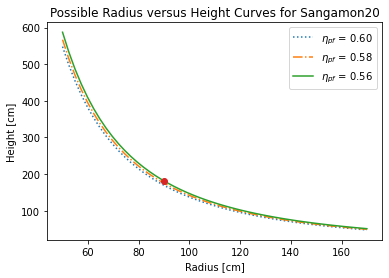
\includegraphics[width = 10cm]{figures/act-core-RH.png}
\caption{Curve of Possible Height and Radii by Packing Fraction}
\label{fig:rh-vol}
\end{figure}

The most critical configurations for a cylinder are either a \emph{square} shape, in which the height is equal to the diameter, or a \emph{flat} shape in which diameter is significantly greater than height.  As a flat shape is disadvantageous for a thermal reactor, the former is chosen.  The point indicated in \ref{fig:rh-vol} shows the radius and height selected for Sangamon20 - a radius of 90 cm, and a height of 180 cm.

\subsection{Graphite Reflector Thickness Determination}

The reflector must be sufficiently thick to keep the reactor critical, and protect the pressure vessel.  To ensure this, the outward current must be less than or equal to the outward current in Sangamon200 at the outer reflector boundary.  The detector layout in Sangamon20 is identical to \ref{fig:det-place}.

\section{Fuel Composition}

The number of passes the pebble has theoretically experienced determines its isotopic composition.  Seven possible pebble compositions exist, one for each of the six 6-month passes, plus an additional composition for fresh pebbles.  The seven pebble compositions are represented equally in number in the core, and they are randomly distributed throughout the core.

The exact isotopic composition is approximated by running a burnup calculation using Serpent2 for a single pebble in a cube.  It uses a reflective boundary condition to simulate the presence of other pebbles or the reflector.  The void in the square is filled with helium.  While the full-core models homogenize the pebbles, the single-pebble burnup model individually models each TRISO particle.  Just as with the location of the pebbles in the full core, the Serpent2 particle dispersal routine generated the TRISO particle locations.

\begin{figure}[H]
\centering
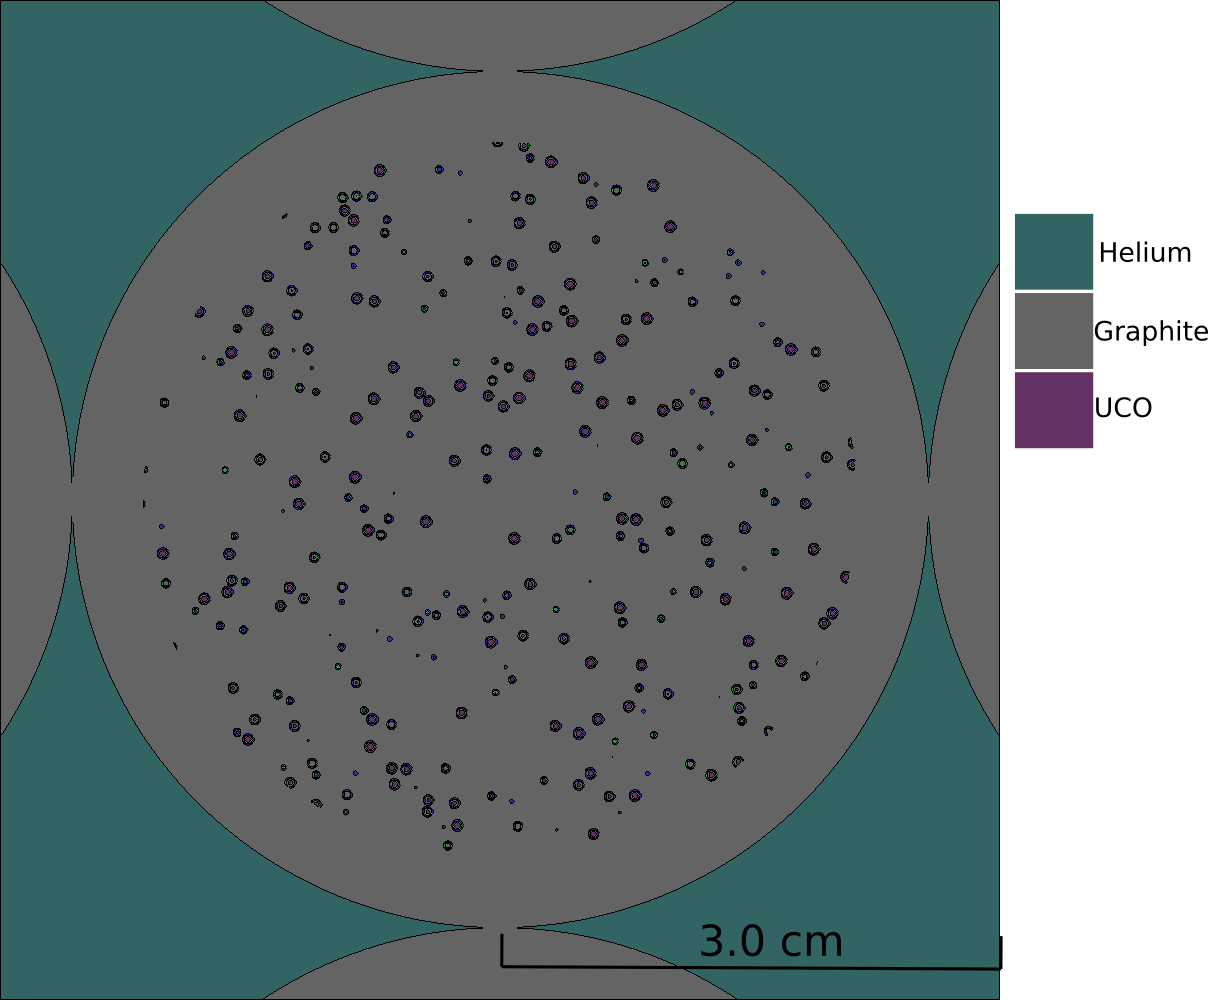
\includegraphics[width = 10cm]{figures/burn-20.png}
\caption{Geometry of the Single-Pebble Burnup Calculation for Sangamon20}
\label{fig:burn-20}
\end{figure}

Once the isotopic compositions are determined, the pebbles are homogenized by volume, to improve performance.  The volume of a TRISO particle, and more specifically, a UCO kernel, is assumed constant.

\section{Reactor Sensitivity to Pebble Locations and Symmetry}

As the pebble locations and compositions are determined randomly, it is entirely possible to have bands in the reactor where multiple pebbles of same (or similar) burnup form lines or pockets.  In the interest of better characterizing the neutronics of the reactor, a sensitivity analysis tested various pebble composition locations.  The \emph{shuffling} test maintained the pebble locations, but changed what composition the individual pebbles were.  A second test completely changed the location of the pebbles in the core by randomly dispersing them again.  The third analyzed the effects of utilizing a symmetry simplification, in order to improve computational speed.  The core was approximated using a $\frac{1}{6}$ slice.  The slice used to simplify changed in each test, shown in \ref{fig:slicetest}.  In each test, all other parameters remain the same.

\begin{figure}[h!]
\centering

\includegraphics[width=0.6\linewidth]{figures/run-layout.png}
\caption{Symmetry Test Run Layouts}
\label{fig:slicetest}
\end{figure}